% -*- coding: utf-8 -*-
%XeLaTeX编译
\documentclass[12pt]{article}
\usepackage{ctex}					%使用中文字体
\usepackage{titlesec}   			%字体宏包
\usepackage[a4paper]{geometry} % 调整纸张大小和页边距的包,中括号中规定了纸张大小
\usepackage{url}					%插入超链接
\usepackage{graphicx}	           %插入图片
 \usepackage{float}				%图片紧跟文字
\usepackage{hyperref}			%目录超链接
%代码段设置
\usepackage{listings}
\usepackage{xcolor}
\lstset{
	numbers=left, 
	numberstyle= \tiny, 
	keywordstyle= \color{ blue!70},
	commentstyle= \color{red!50!green!50!blue!50}, 
	frame=shadowbox, % 阴影效果
	rulesepcolor= \color{ red!20!green!20!blue!20} ,
	escapeinside=``, % 英文分号中可写入中文
	xleftmargin=2em,xrightmargin=2em, aboveskip=1em,
	basicstyle=\footnotesize,
	%framexleftmargin=2em
  %  backgroundcolor=\color{red!50!green!50!blue!50},%代码块背景色为浅灰色
	breaklines=true,  %代码过长则换行
}

\geometry{left=2.0cm,right=2.0cm,top=2.0cm,bottom=2.0cm} % 页边距设置

\begin{document}
    \begin{titlepage}
        \heiti
        \vspace*{64pt}
        \begin{center}
            \fontsize{72pt}{0} 实验二\\
            \vspace*{36pt}
            \fontsize{48pt}{0}{实\quad 验\quad 报\quad 告}\\
            \vspace*{48pt}
    
            \vspace*{48pt}
        
            \LARGE 学院\ \ \underline{\makebox[200pt]{数据科学与计算机学院}}\\
            \LARGE 专业\ \ \underline{\makebox[200pt]{计算机类}}\\
			 \LARGE 年级\ \ \underline{\makebox[200pt]{18级}}\\
			 \LARGE 姓名\ \ \underline{\makebox[200pt]{黄思蓉}}\\
			\LARGE 学号\ \ \underline{\makebox[200pt]{18340064}}\\
			\LARGE 课程名称\ \ \underline{\makebox[200pt]{操作系统原理实验}}\\
            \vspace*{72pt}
        \end{center}
    \end{titlepage}

\newpage

\tableofcontents   % 生成目录
\newpage


\section{\LARGE 实验题目}
\large 加载用户程序


\section{\LARGE 实验目的}
\begin{enumerate}
\item 了解监控程序执行用户程序的主要工作
\item 了解一种用户程序的格式与运行要求
\item 加深对监控程序概念的理解
\item 掌握加载用户程序方法
\item 掌握几个BIOS调用和简单的磁盘空间管理
\end{enumerate}


\section{\LARGE 实验要求}
\begin{enumerate}
\item 知道引导扇区程序实现用户程序加载的意义
\item 掌握COM/BIN等一种可执行的用户程序格式与运行要求
\item 将自己实验一的引导扇区程序修改为3-4个不同版本的COM格式程序,每个程序缩小显示区域,在屏幕特定区域显示,用以测试监控程序,在1.44MB软驱映像中存储这些程序
\item 重写1.44MB软驱引导程序,利用BIOS调用,实现一个能执行COM格式用户程序的监控程序
\item 设计一种简单命令,实现用命令交互执行在1.44MB软驱映像中存储几个用户程序
\item 编写实验报告,描述实验工作的过程和必要的细节,如截屏或录屏,以证实实验工作的真实性
\end{enumerate}


\section{\LARGE 实验内容}
\begin{enumerate}
\item 将自己实验一的引导扇区程序修改为一个的COM格式程序,程序缩小显示区域,在屏幕第一个1/4区域显示,显示一些信息后,程序会结束退出,可以在DOS中运行。在1.44MB软驱映像中制定一个或多个扇区,存储这个用户程序a。
相似地、将自己实验一的引导扇区程序修改为第二、第三、第四个的COM格式程序,程序缩小显示区域,在屏幕第二、第三、第四个1/4区域显示,在1.44MB软驱映像中制定一个或多个扇区,存储用户程序b、用户程序c、用户程序d。
\item 重写1.44MB软驱引导程序,利用BIOS调用,实现一个能执行COM格式用户程序的监控程序。程序可以按操作选择,执行一个或几个用户程序。解决加载用户程序和返回监控程序的问题,执行完一个用户程序后,可以执行下一个。
\item 设计一种命令,可以在一个命令中指定某种顺序执行若干个用户程序。可以反复接受命令。
\item 在映像盘上,设计一个表格,记录盘上有几个用户程序,放在那个位置等等信息,如果可以,让监控程序显示出表格信息。
\item 拓展自己的软件项目管理目录,管理实验项目相关文档
\end{enumerate}


\section{\LARGE 实验方案}
\begin{enumerate}
\item 安装虚拟机VirtualBox
\item 获取可视化编辑十六进制文件内容的工具
\item 安装nasm编译器,编译asm文件
\item 学习x86,编辑引导程序代码
\end{enumerate}

\section{\LARGE 实验过程}

	\subsection{\Large 安装虚拟机}
	\paragraph{}登陆官网 \url{https://www.virtualbox.org/wiki/Downloads} ,如下图1点击Windows hosts即可
		\begin{figure}[H]
			%\small
			\centering
			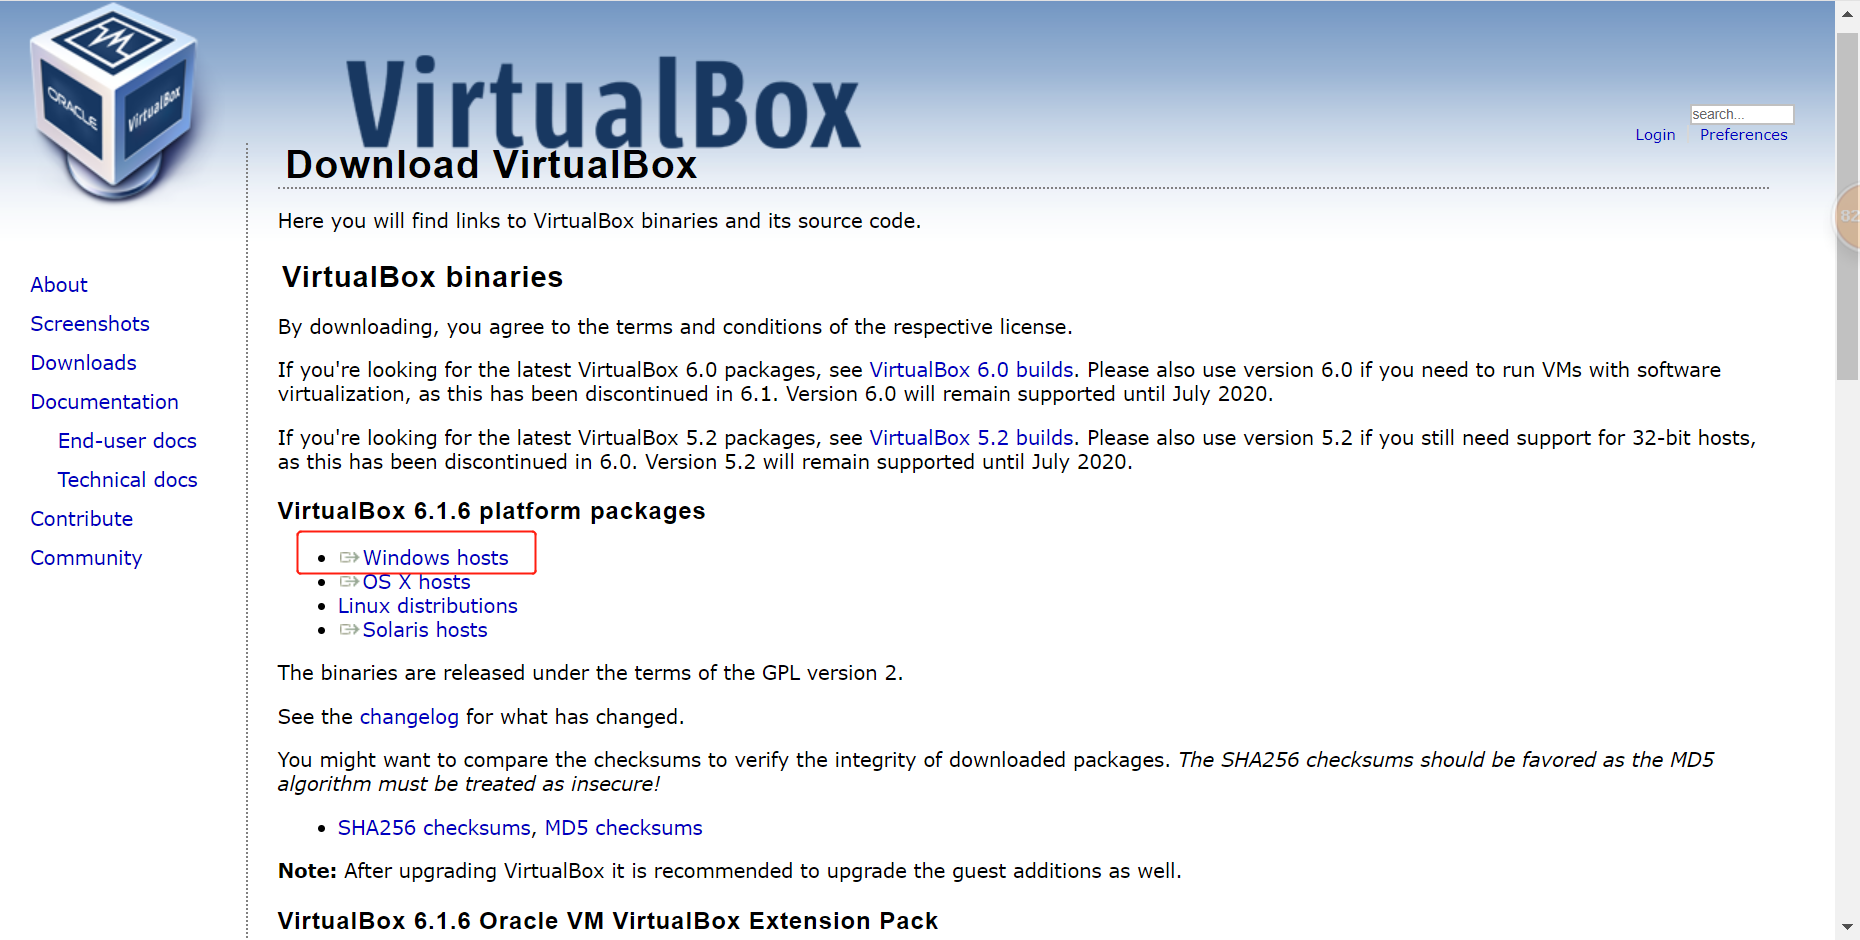
\includegraphics[width=14cm]{./figures/VirtualBoxDownLoad.png}
			\caption{VirtualBox下载} 
		\end{figure}
			\paragraph{}接着是安装过程,直接点击下载好的 VirtualBox-6.1.4-136177-Win.exe 文件,如图2(写此报告时已经安装好虚拟机了)。接着只用一直点击下一步即可。安装过程是参照这篇博客 \url{https://blog.csdn.net/qq_33690342/article/details/81412167} ,安装过程很顺利,在这里不赘述。
		\begin{figure}[H]
			%\small
			\centering
			
\includegraphics[width=14cm]{./figures/VirtualBoxEXE.png}
			\caption{VirtualBox安装} 
		\end{figure}
		\begin{figure}[H]
			%\small
			\centering
			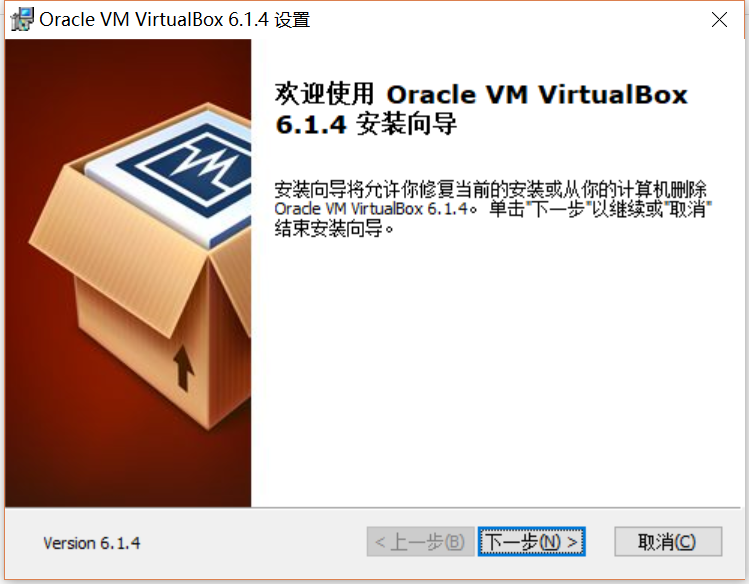
\includegraphics[width=12cm]{./figures/VirtualBoxInstall.png}
			\caption{VirtualBox安装过程} 
		\end{figure}


	\subsection{\Large 获取可视化编辑十六进制文件内容的工具}
	\paragraph{}登陆winhex官网下载即可 \url{https://winhex.en.softonic.com/} ,另外也可以获取李忠老师的《 x86 汇编语言-从实模式到保护模式》这本书的配套工具HexView,不过该工具只能查看不能编辑保存。
		\begin{figure}[H]
			%\small
			\centering
			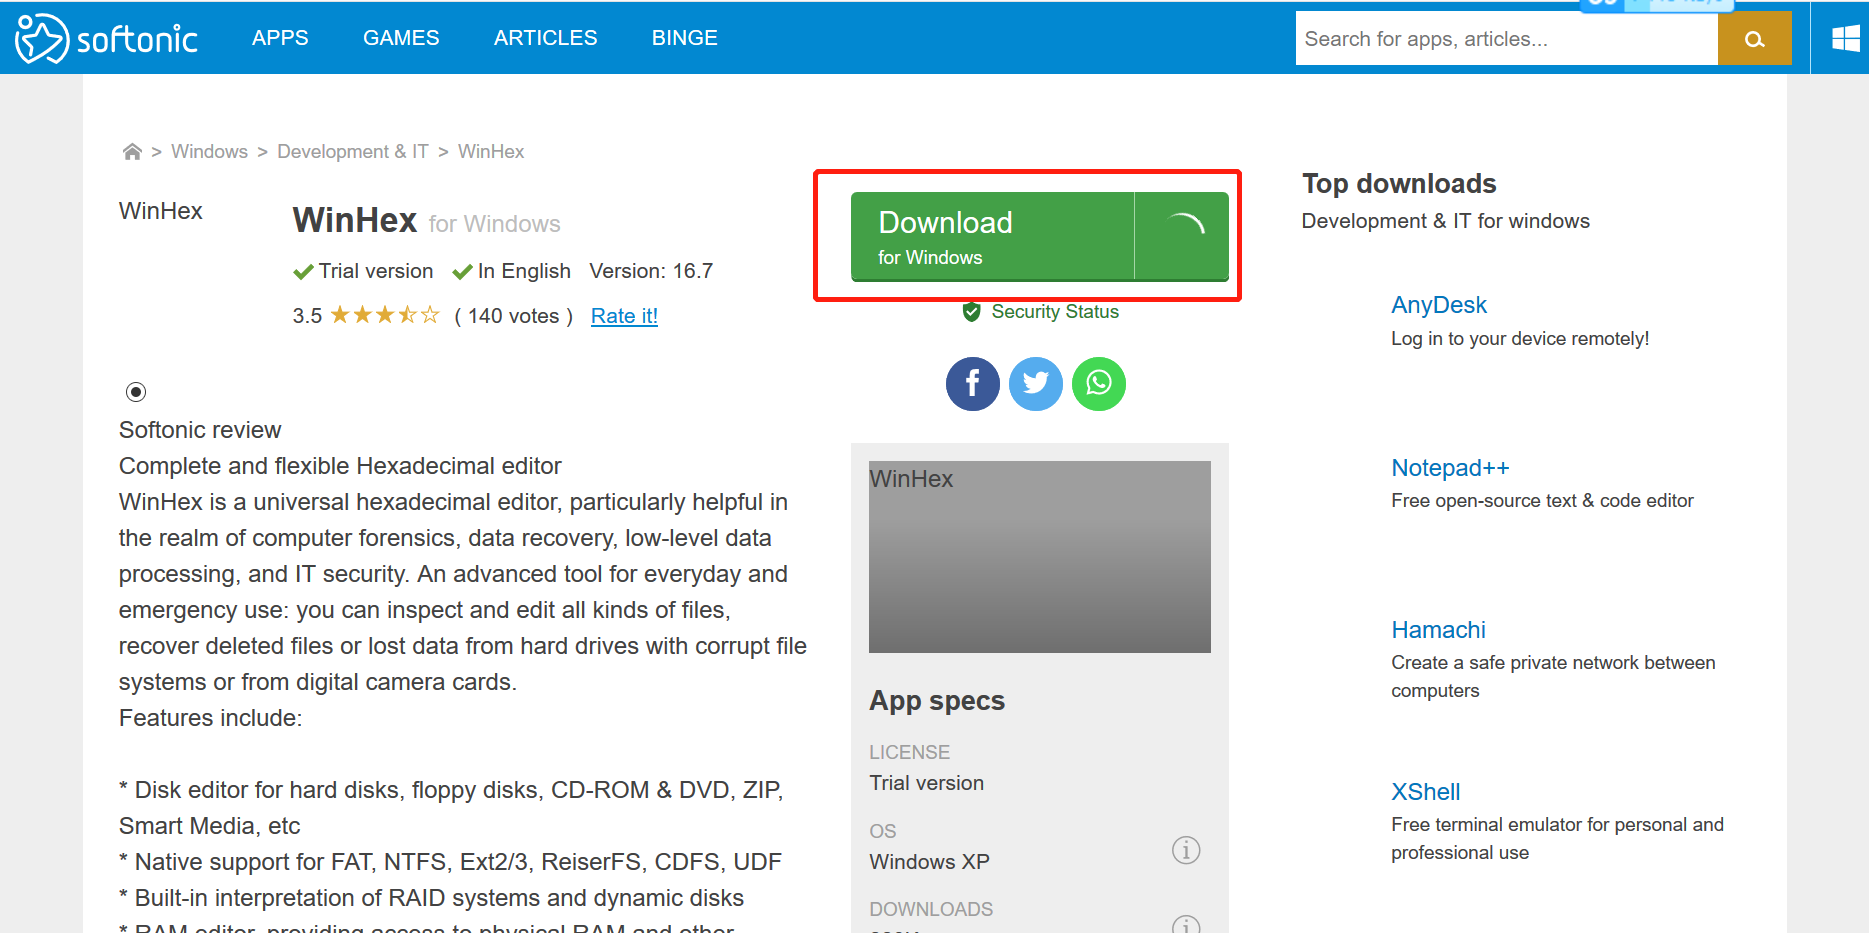
\includegraphics[width=14cm]{./figures/WinHex.png}
			\caption{WinHex下载} 
		\end{figure}
		\begin{figure}[H]
			%\small
			\centering
			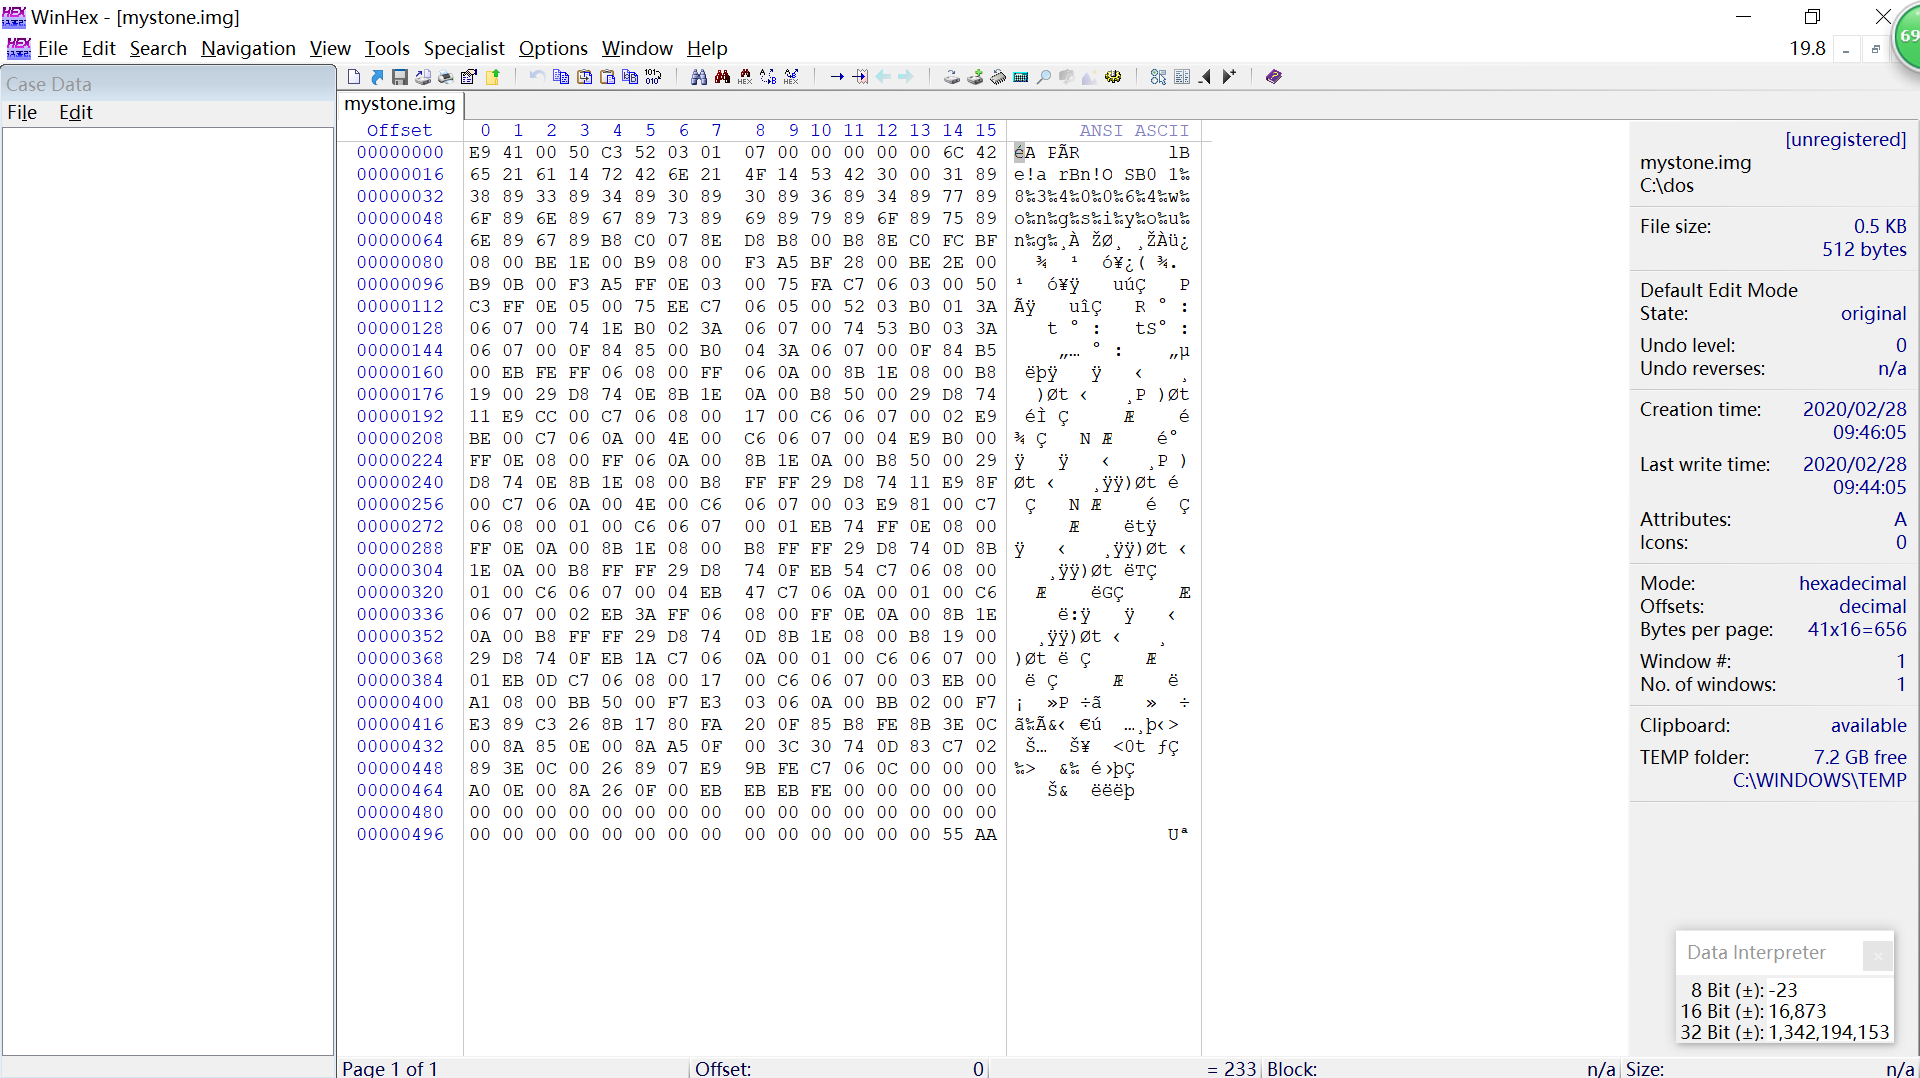
\includegraphics[width=14cm]{./figures/winhexuse.png}
			\caption{WinHex使用示意} 
		\end{figure}
		\begin{figure}[H]
			%\small
			\centering
			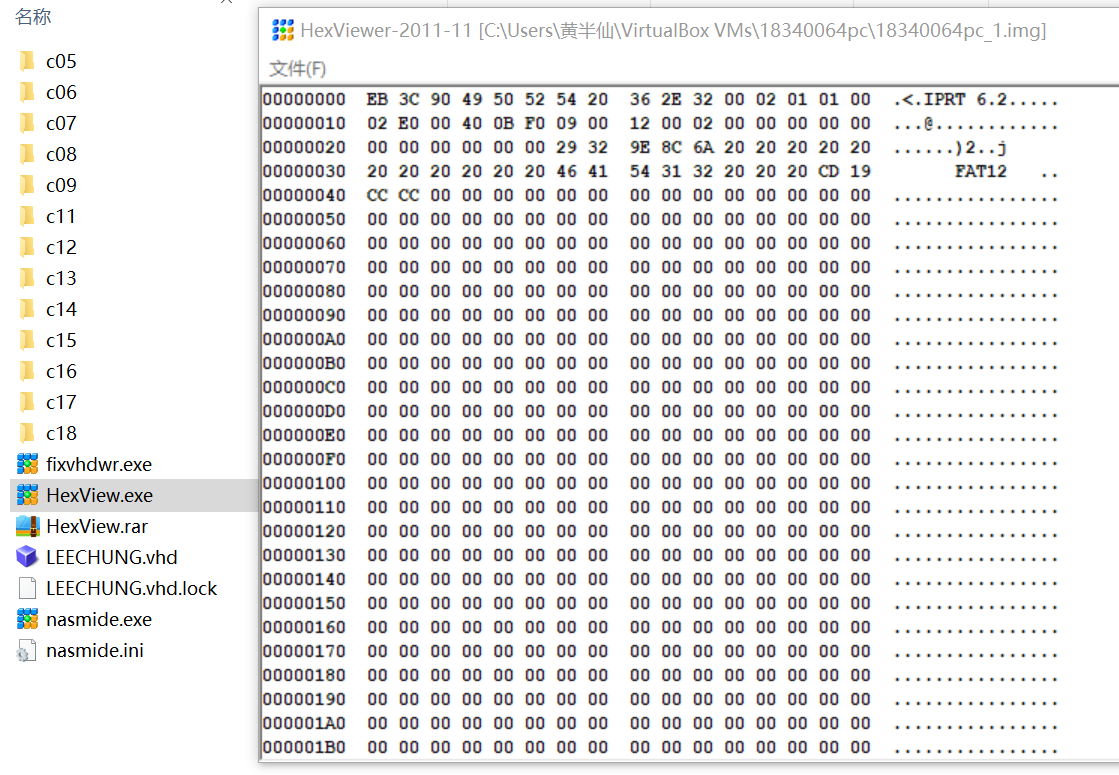
\includegraphics[width=12cm]{./figures/HexViewer.png}
			\caption{HexView使用示意} 
		\end{figure}


	\subsection{\Large 安装nasm}
	\paragraph{}同样地登陆nasm官网 \url{https://www.nasm.us/} ,点击DOWNLOAD,选择合适的版本下载,我选择的是nasm-2.11.02-installer
		\begin{figure}[H]
			%\small
			\centering
			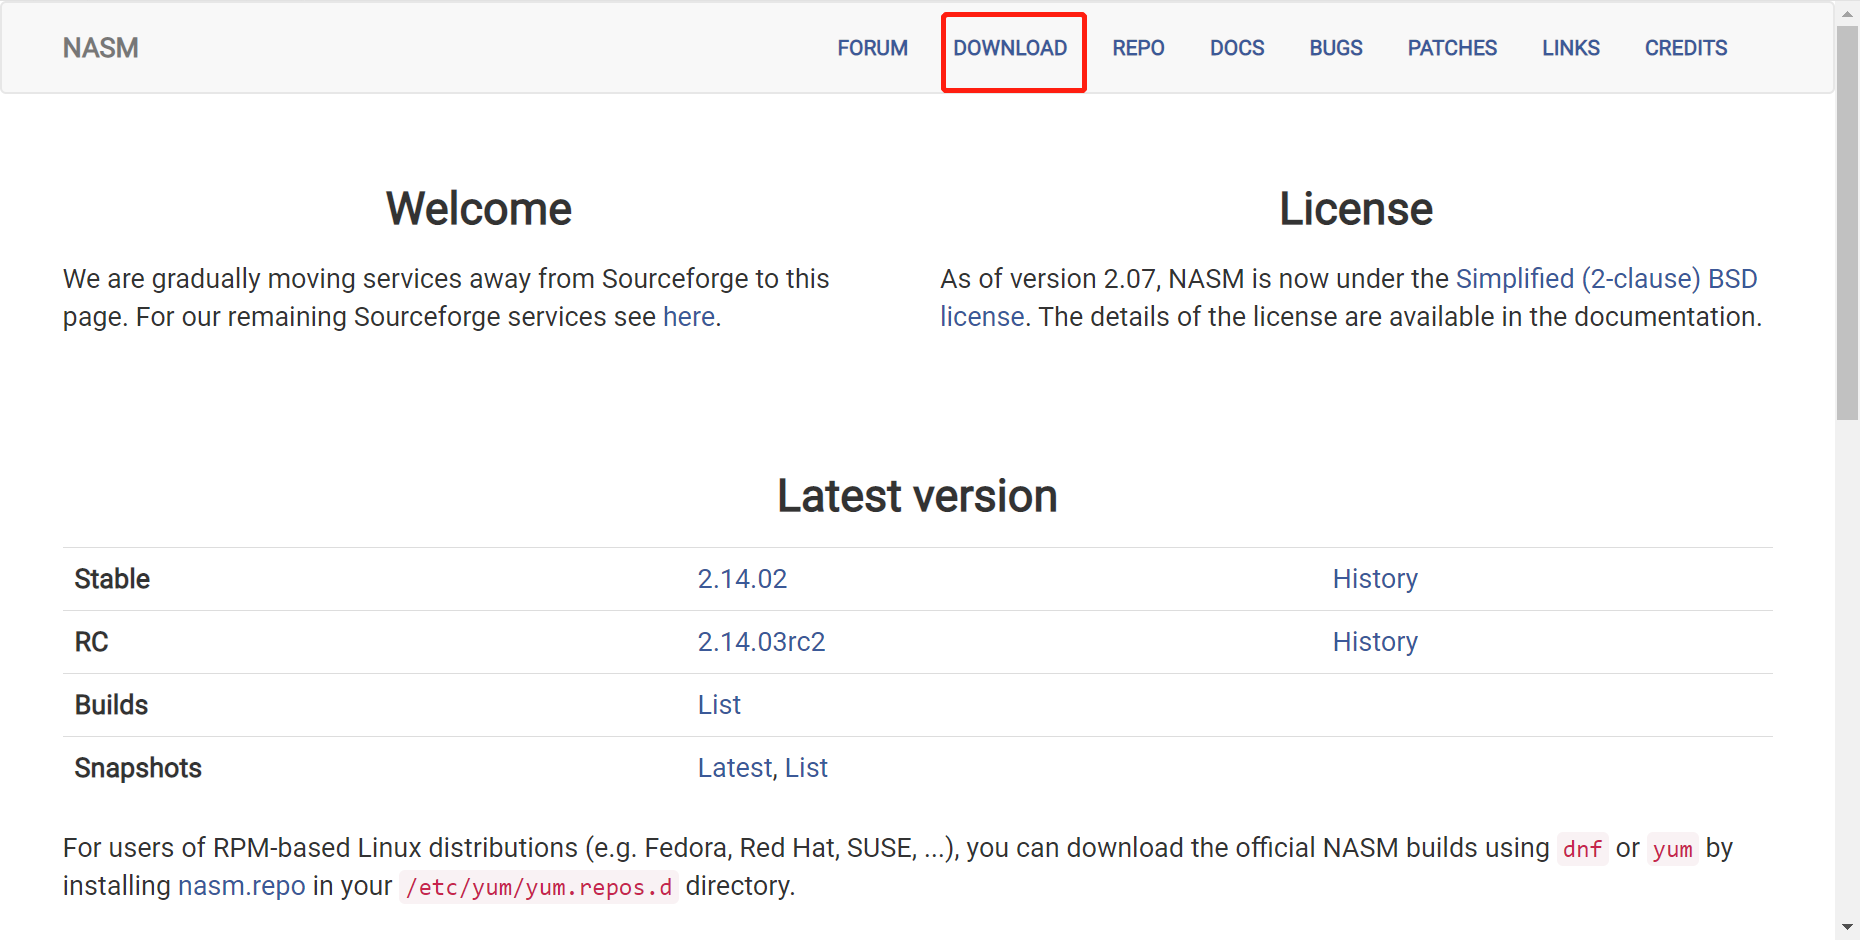
\includegraphics[width=14cm]{./figures/NASMD.png}
			\caption{NASM下载} 
		\end{figure}

		\begin{figure}[H]
			%\small
			\centering
			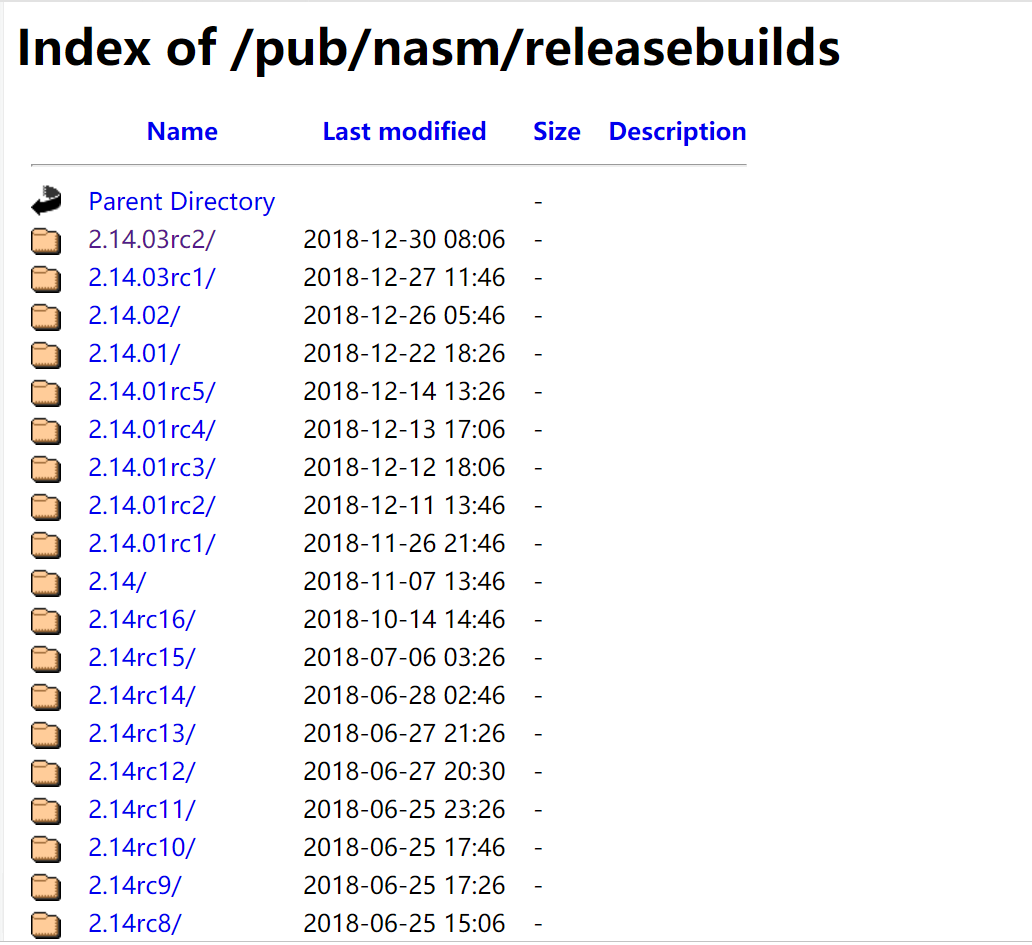
\includegraphics[width=14cm]{./figures/NASMD3.png}
			\caption{NASM下载} 
		\end{figure}

		\begin{figure}[H]
			%\small
			\centering
			\includegraphics[width=14cm]{./figures/NASMD2.png}
			\caption{NASM下载} 
		\end{figure}


	\paragraph{}下面是安装过程,双击从官网下载的exe文件,也是只用点击next,直到出现install按钮即可,其中可以改变文件安装路径。
		\begin{figure}[H]
			%\small
			\centering
			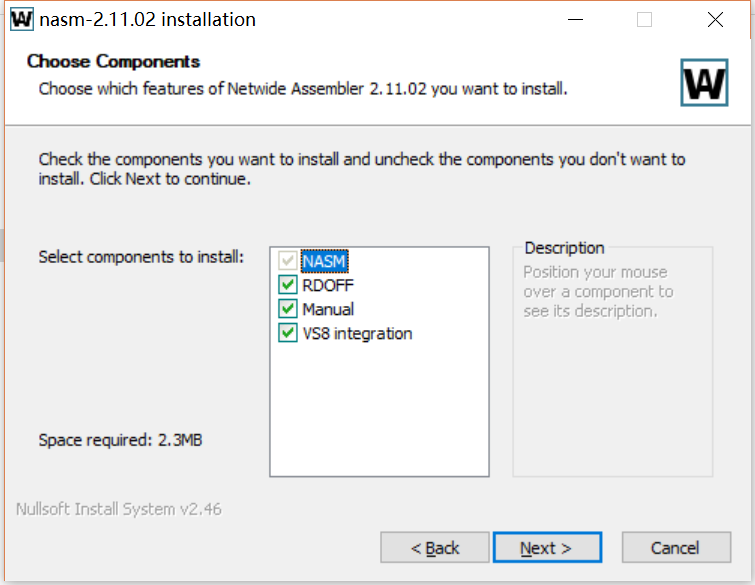
\includegraphics[width=14cm]{./figures/Install1.png}
			\caption{NASM安装} 
		\end{figure}	

	\paragraph{}安装成功如图:
		\begin{figure}[H]
			%\small
			\centering
			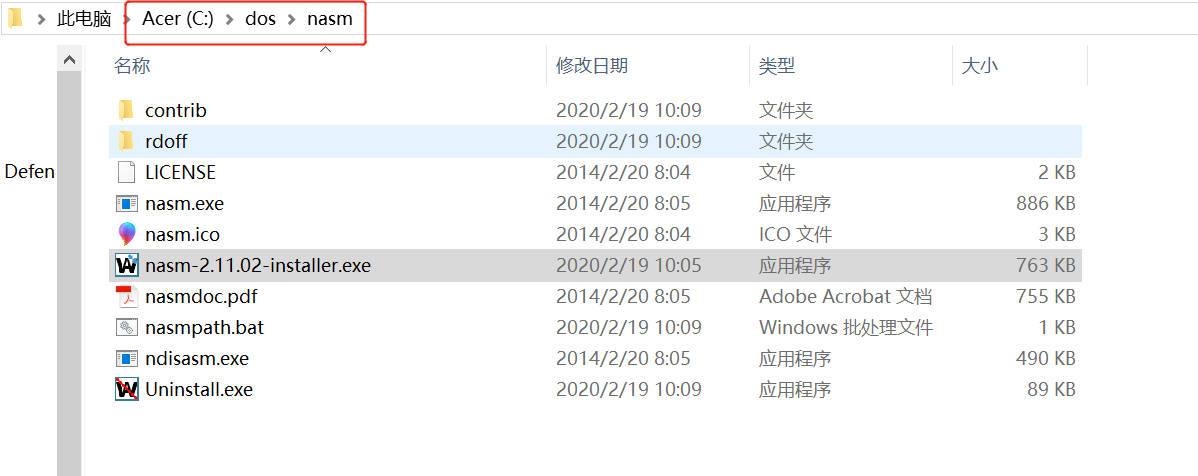
\includegraphics[width=14cm]{./figures/Install3.png}
			\caption{NASM安装完毕} 
		\end{figure}	

	\paragraph{}为了方便使用,配置环境变量:
		\begin{figure}[H]
			%\small
			\centering
			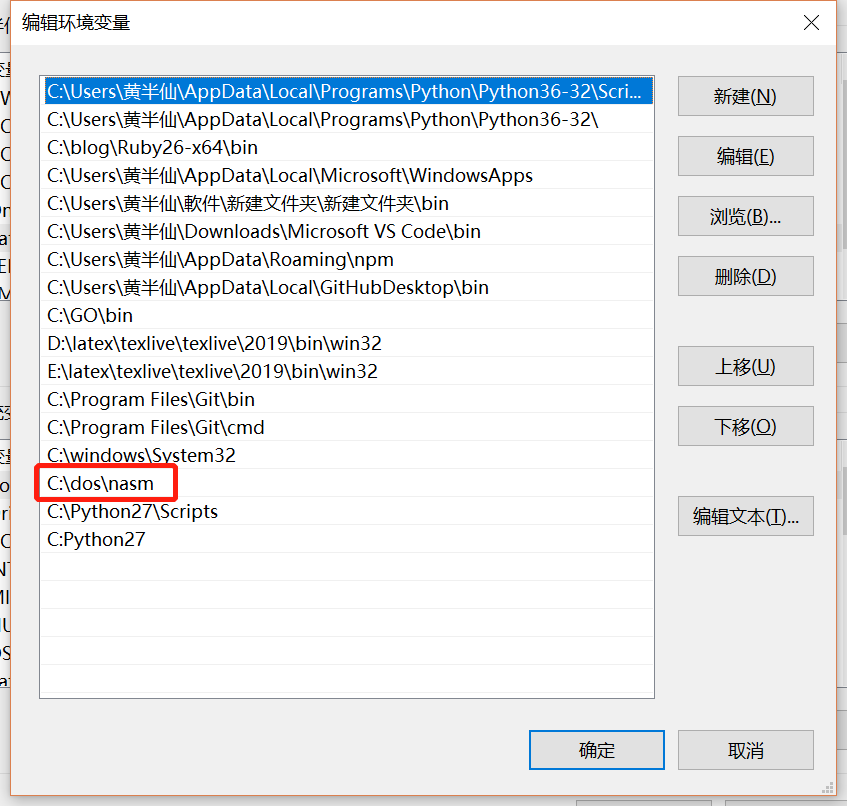
\includegraphics[width=10cm]{./figures/Environemt.png}
			\caption{配置环境变量} 
		\end{figure}	
\vspace*{7pt}
	\paragraph{}在命令窗口输入nasm -v命令检验
		\begin{figure}[H]
			%\small
			\centering
			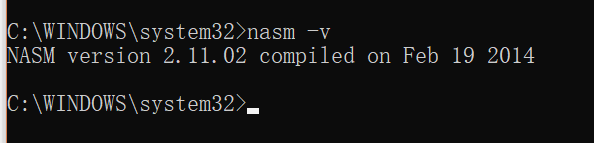
\includegraphics[width=14cm]{./figures/cmd.png}
			\caption{nasm -v命令} 
		\end{figure}

	\subsection{\Large 编辑引导程序代码}
	\paragraph{}老师提供的代码其实已经实现了以字符‘A’作运动轨迹,但是编译失败,只用稍微改一下下面的代码就可以了!其中ds指向地址0x7c00,因为bios执行完后,cpu从这里开始执行指令;es指向0B800h,因为在内存地址空间中,B800h\~{}BFFFFh共32KB的空间,为80x25彩色字符模式的显示缓冲区。

		\begin{figure}[H]
			%\small
			\centering
			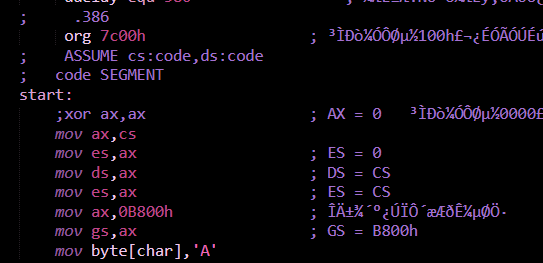
\includegraphics[width=14cm]{./figures/teachercode.png}
			\caption{老师提供的部分代码} 
		\end{figure}	

		\begin{figure}[H]
			%\small
			\centering
			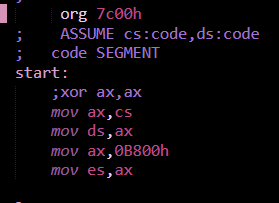
\includegraphics[width=10cm]{./figures/alter1.png}
			\caption{一种修改方式} 
		\end{figure}	


		\begin{figure}[H]
			%\small
			\centering
			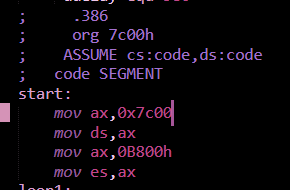
\includegraphics[width=10cm]{./figures/alter2.png}
			\caption{另一种修改方式} 
		\end{figure}	

	\paragraph{}接着修改数据段,增加个人信息:学号(18340064),姓名(huangsirong),根据显示原理:低位字节存储字符的ASCII码,高位字节存储字符的属性,属性字节格式:		
	\begin{figure}[H]
			%\small
			\centering
			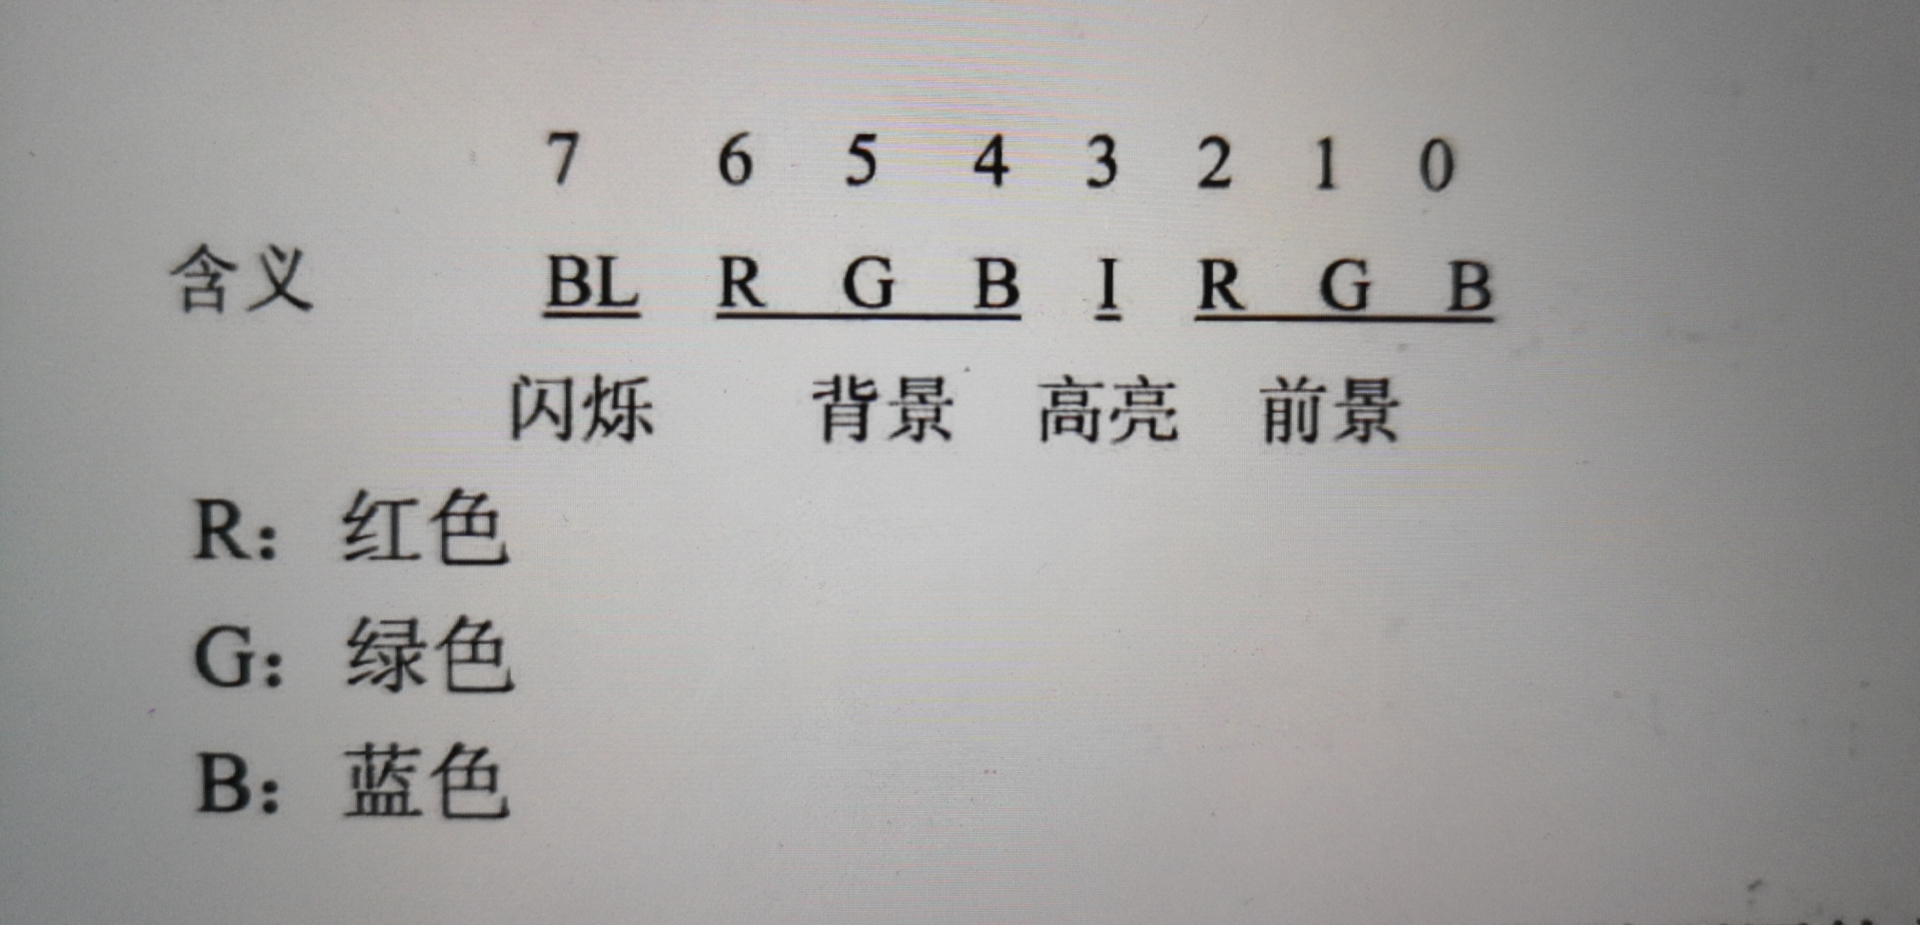
\includegraphics[width=10cm]{./figures/ascii.jpg}
			\caption{字符属性} 
		\end{figure}	

	\begin{lstlisting}
datadef:	
    count dw delay		;延迟计时
    dcount dw ddelay		;延迟计时
    rdul db Dn_Rt			;运动方向
    x    dw 7		;行位置
    y    dw 0		;列位置
    cnt  dw 0		;计数器
    char db 'l',42h,'e',21h,'a',14h,'r',42h,'n',21h,'O',14h,'S',42h,'0',0		;要显示的字符
    number  db	'1',89h,'8',89h,'3',89h,'4',89h,'0',89h,'0',89h,'6',89h,'4',89h  ;要显示的学号
    name	db 'h',89h,'u',89h,'a',89h,'n',89h,'g',89h,'s',89h,'i',89h,'r',89h,'o',89h,'n',89h,'g',89h ;要显示的姓名拼音
	\end{lstlisting}

	\paragraph{}在开始以蛇形运动轨迹显示"learnos"之前,显示个人信息:
	\begin{lstlisting}
showmeg:
	cld
	mov	di,8	 		;指定显示屏的位置
	mov si,number     ;指向要显示的学号
	mov cx,8          ;8位学号,循环8次
	rep movsw
	mov di,28h  		;指定显示屏的位置
	mov si,name       ;指向要显示的姓名拼音
	mov cx,11         ;循环11次
	rep movsw
	\end{lstlisting}

   \paragraph{}为了避免learnos在显示过程中覆盖了已显示的姓名学号,修改show部分的程序,避开:
\begin{lstlisting}
show:	
    mov ax,word[x]	    ;word[x]当前行
	mov bx,80
	mul bx;				;word[x]*80
	add ax,word[y]			;行+列=当前位置
	mov bx,2
	mul bx			;2*(行+列),一个字符显示占两个字节
	mov bx,ax				;计算结果ax送给bx

	mov dx,[es:bx]			;获得当前显示屏的字符ascii码
	cmp dl,' '		;如果为空,就显示,否则直接进入下一次循环,跳过本次显示
	jnz loop1				;避开显示的信息

	mov di,[cnt]			;循环显示"learnos"的计数
	mov al,byte[char+di]	;要显示的字符
	mov ah,byte[char+di+1]	;设置字符属性

	cmp al,'0'				;"learnos"末尾标志
	jz s1

	add di,2				;指向下一次要显示的字符,2个字节
	mov [cnt],di			;存储下一次要显示的字符的偏移量
		
con:
	mov [es:bx],ax  		;送入显示器
	jmp loop1				;继续蛇形运动

s1:
	mov word[cnt],0			;重新循环"learnos"
	mov al,byte[char]		;要显示的字符
	mov ah,byte[char+1]		;设置字符属性
	jmp con
\end{lstlisting}

	\paragraph{}至此,在老师提供的代码上编辑完毕,用nasm命令编译该程序,在终端输入命令nasm xxx.asm -o xxx.img 即可
	\begin{figure}[H]
			%\small
			\centering
			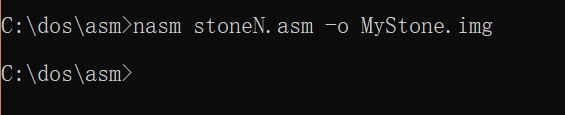
\includegraphics[width=10cm]{./figures/asembly.png}
			\caption{编译} 
		\end{figure}	

	\begin{figure}[H]
			%\small
			\centering
			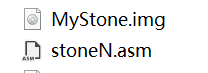
\includegraphics[width=10cm]{./figures/success.png}
			\caption{编译结果} 
		\end{figure}	

	\paragraph{}获得img映像文件后,使用winhex打开,可以看到有512字节且以0x55aa结尾,是可引导程序,缘于代码:
	\begin{lstlisting}
times 510-($-$$) db 0
 db 0x55,0xaa	
	\end{lstlisting}
只要前面的代码量不超多510字节就可以。接着用winhex写入利用虚拟机生成的1.44MB的软盘映像文件中

	\begin{figure}[H]
			%\small
			\centering
			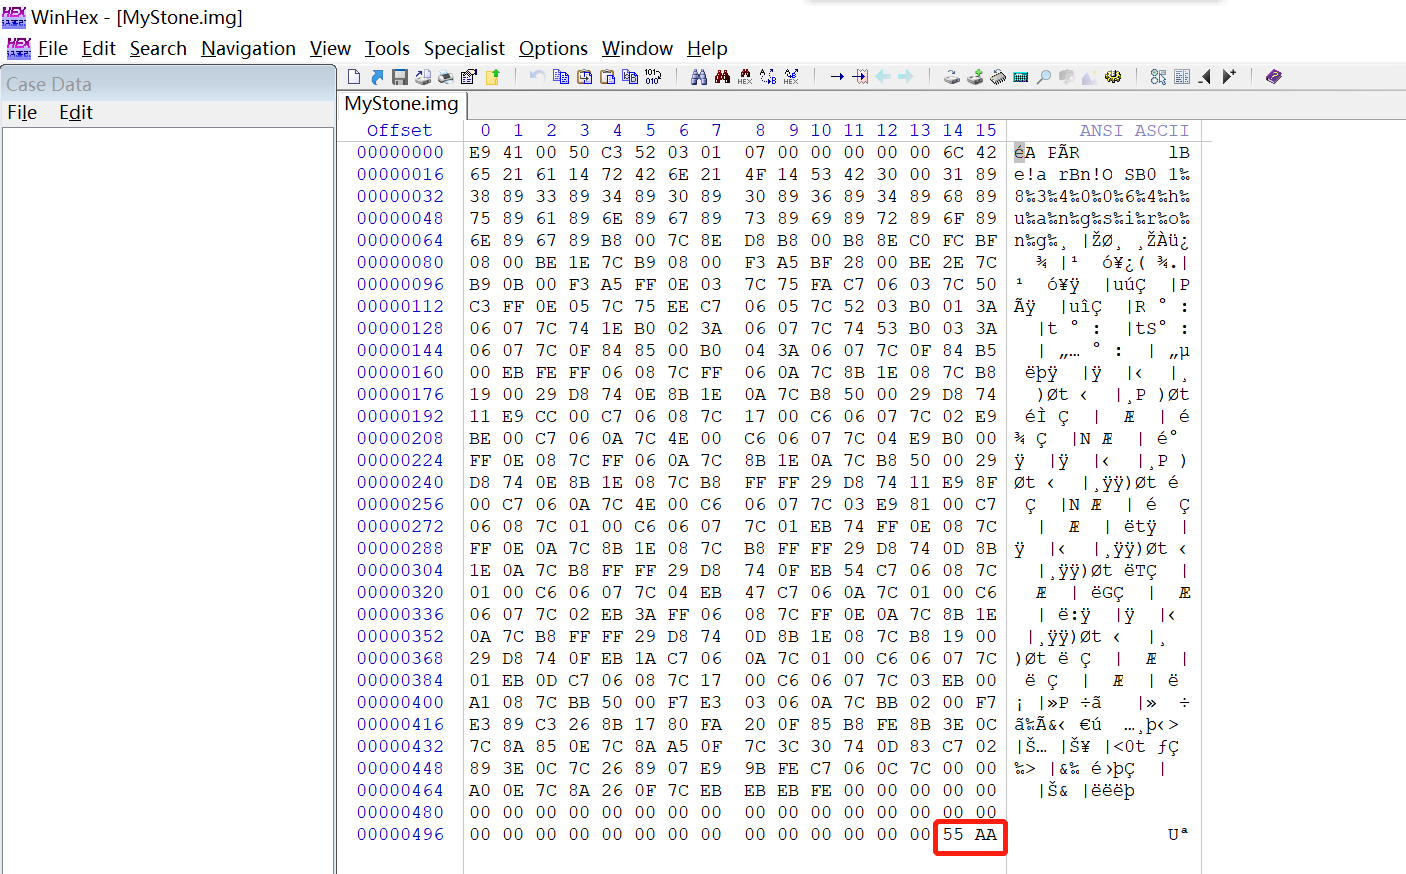
\includegraphics[width=14cm]{./figures/55aa.png}
			\caption{MyStone} 
		\end{figure}	


	\subsection{\Large 创建虚拟机,生成3个1.44MB的软盘映像文件}
\paragraph{}打开VirtualBox,点击新建	
	\begin{figure}[H]
			%\small
			\centering
			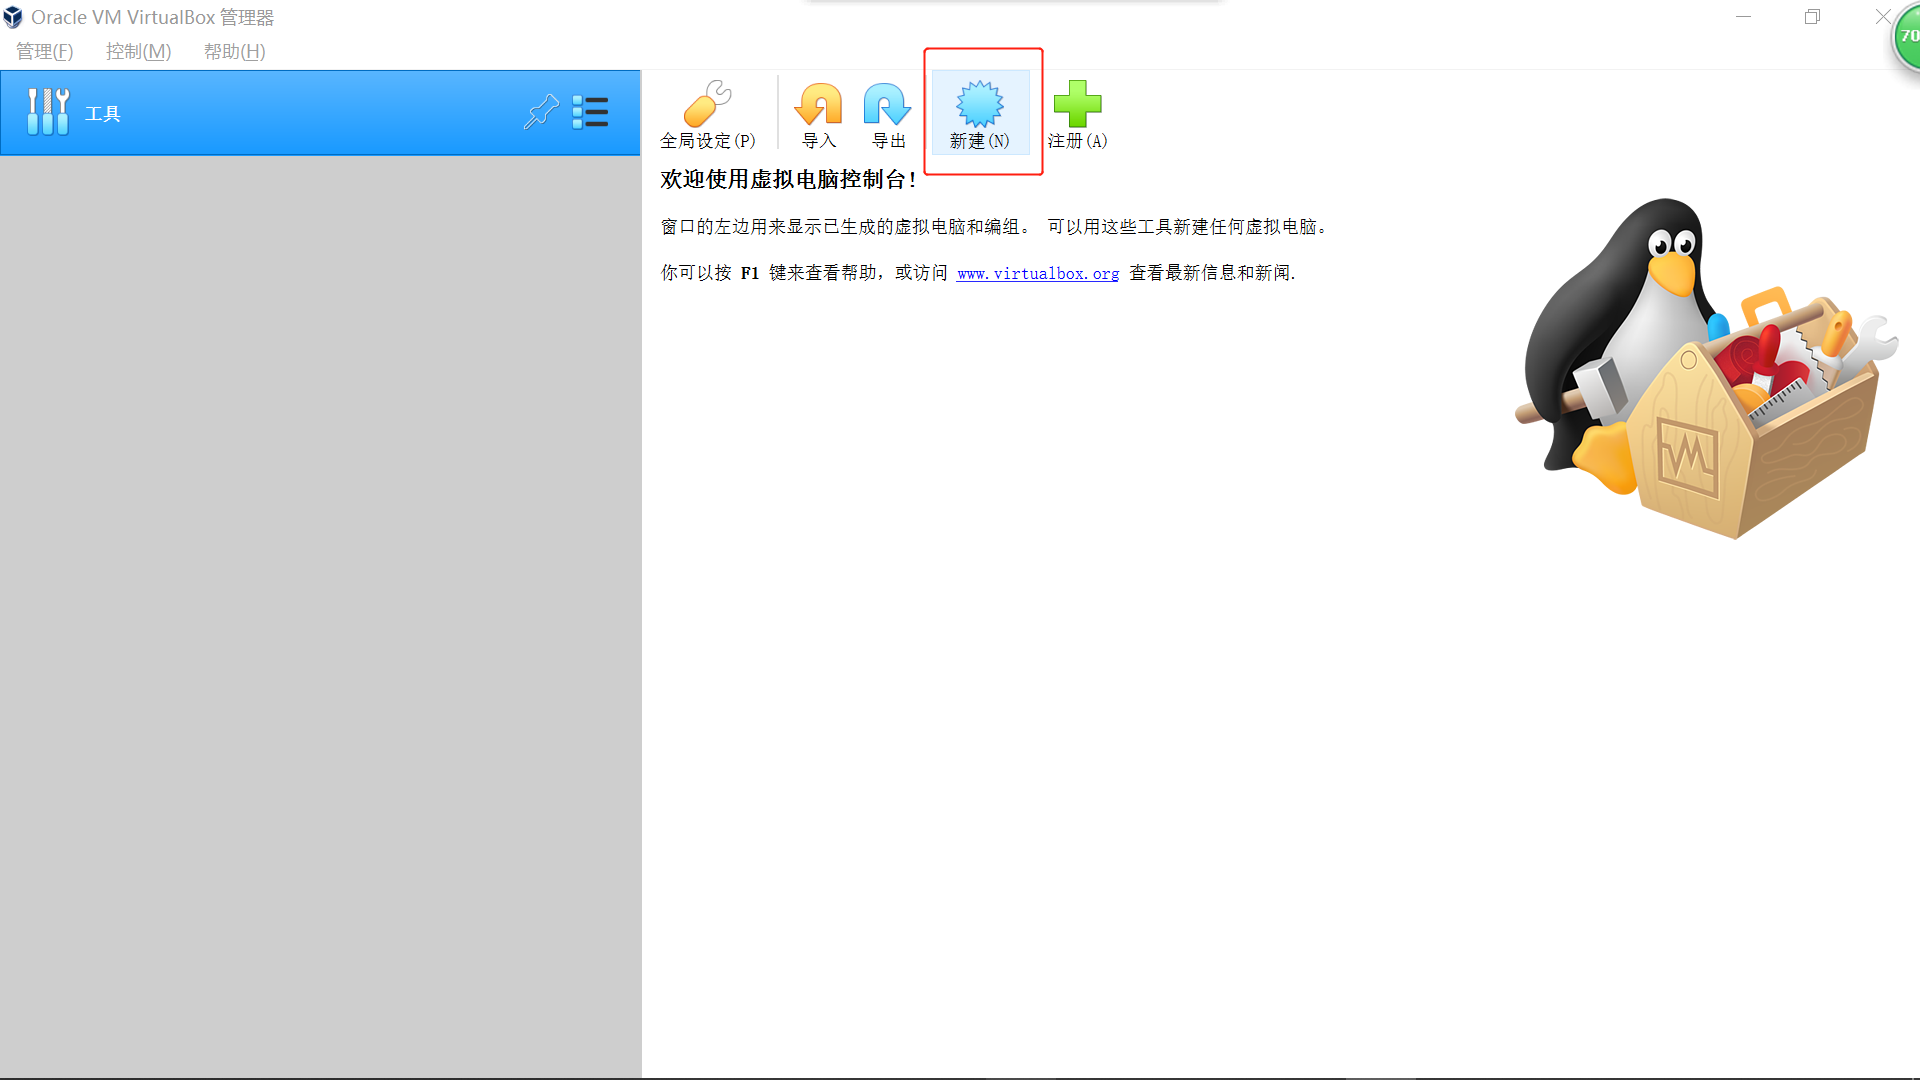
\includegraphics[width=14cm]{./figures/open.png}
			\caption{新建虚拟机} 
		\end{figure}	
设置虚拟机信息:
	\begin{figure}[H]
			%\small
			\centering
			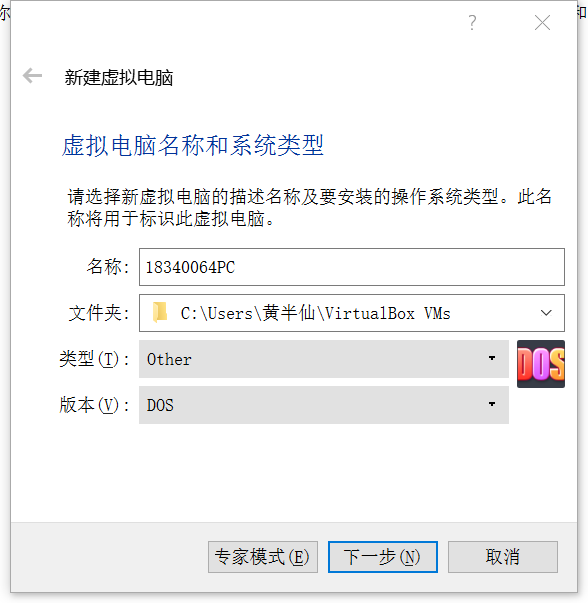
\includegraphics[width=8cm]{./figures/create.png}
			\caption{设置虚拟机名字,类型} 
		\end{figure}	

创建软盘映像文件,按照老师的要求,创建三个映像文件分别为dos格式化软盘,写自己信息的软盘,写入引导程序的软盘,如下面的图展示dos创建过程,其余两个也是一样的步骤,分别命名为:dos.img , Message.img , boot.img
	\begin{figure}[H]
			%\small
			\centering
			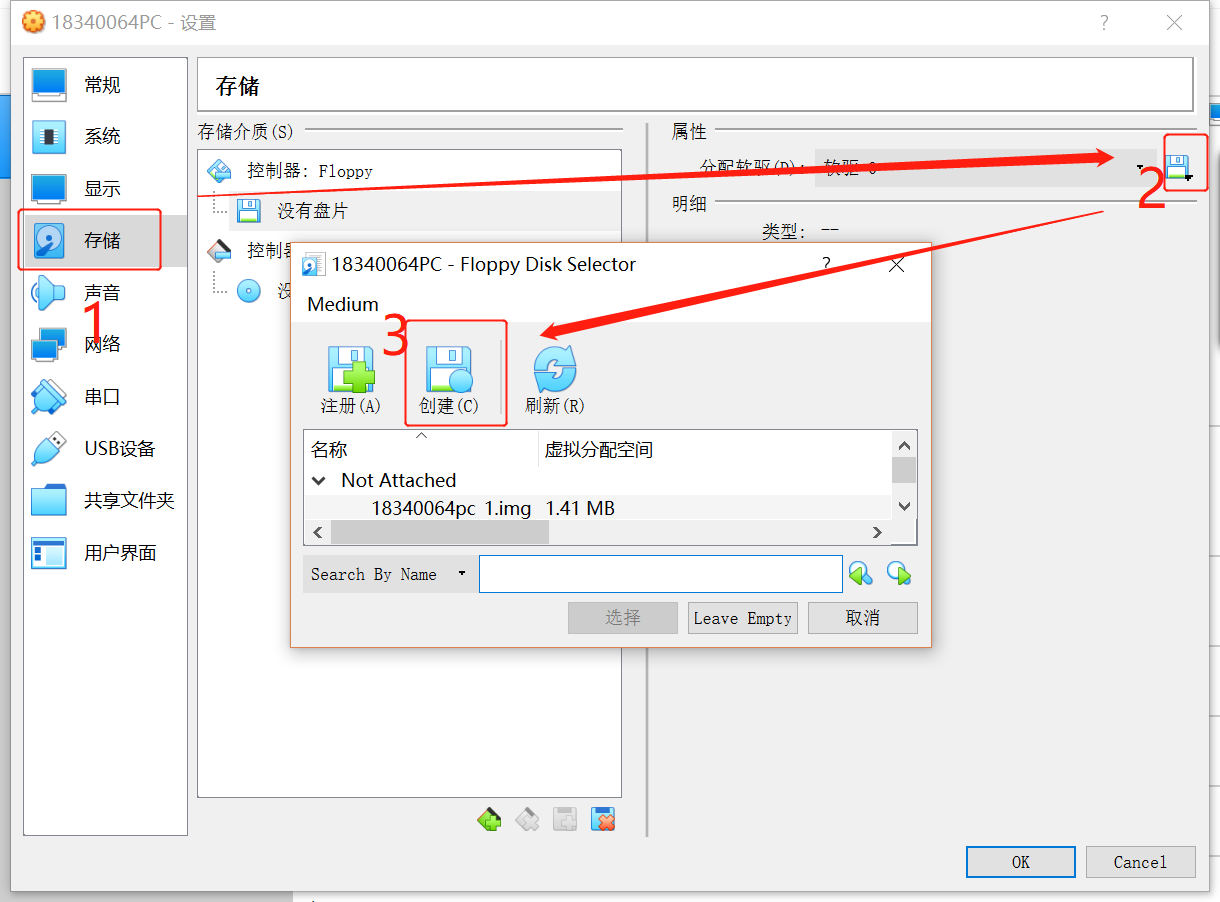
\includegraphics[width=8cm]{./figures/createimg.png}
			\caption{创建dos映像文件} 
		\end{figure}	

	\begin{figure}[H]
			%\small
			\centering
			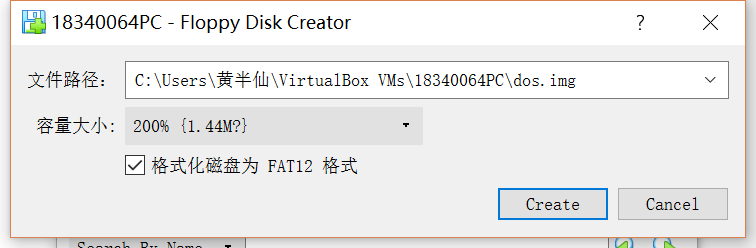
\includegraphics[width=8cm]{./figures/dos.png}
			\caption{创建dos映像文件} 
		\end{figure}	

然后将刚刚生成的MyStone.img文件的512字节写入boot.img的第一个512字节中。本来是用前面写的winhex来修改的,但是winhex显示boot.img文件超过200kb无法修改,后来直接用sublime打开,也可以修改保存
	\begin{figure}[H]
			%\small
			\centering
			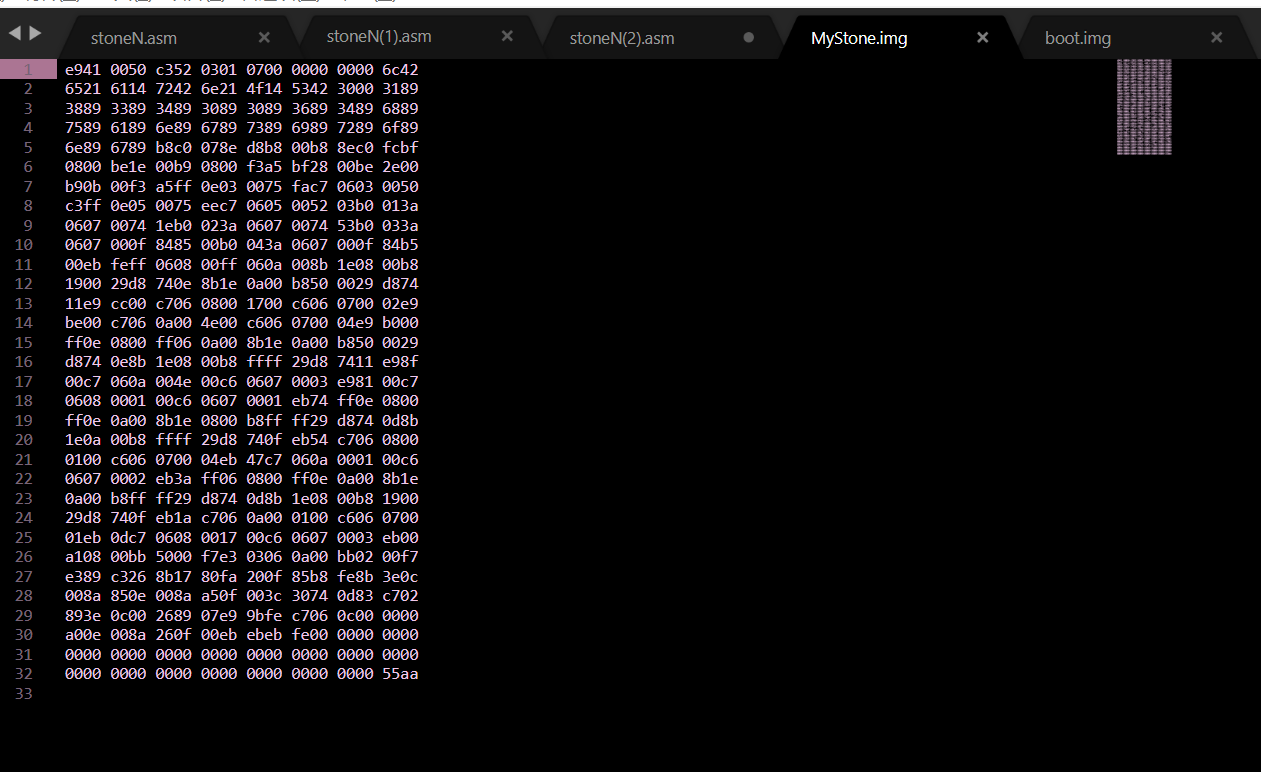
\includegraphics[width=10cm]{./figures/MyStone.png}
			\caption{MyStone文件} 
		\end{figure}	

	\begin{figure}[H]
			%\small
			\centering
			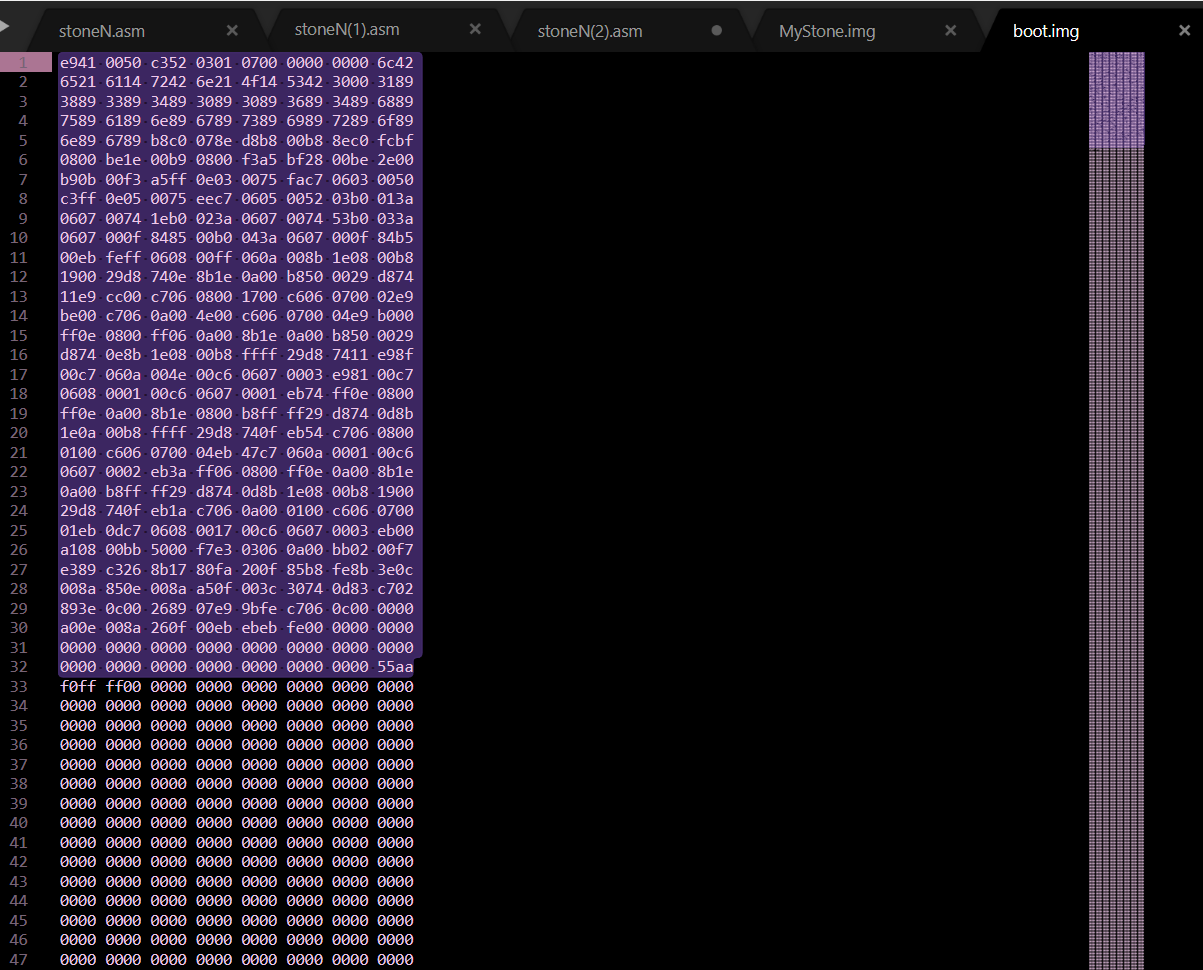
\includegraphics[width=12cm]{./figures/boot.png}
			\caption{boot文件} 
		\end{figure}	

设置虚拟机软驱为刚刚改动的boot.img,然后开机启动,结果如下:
	\begin{figure}[H]
			%\small
			\centering
			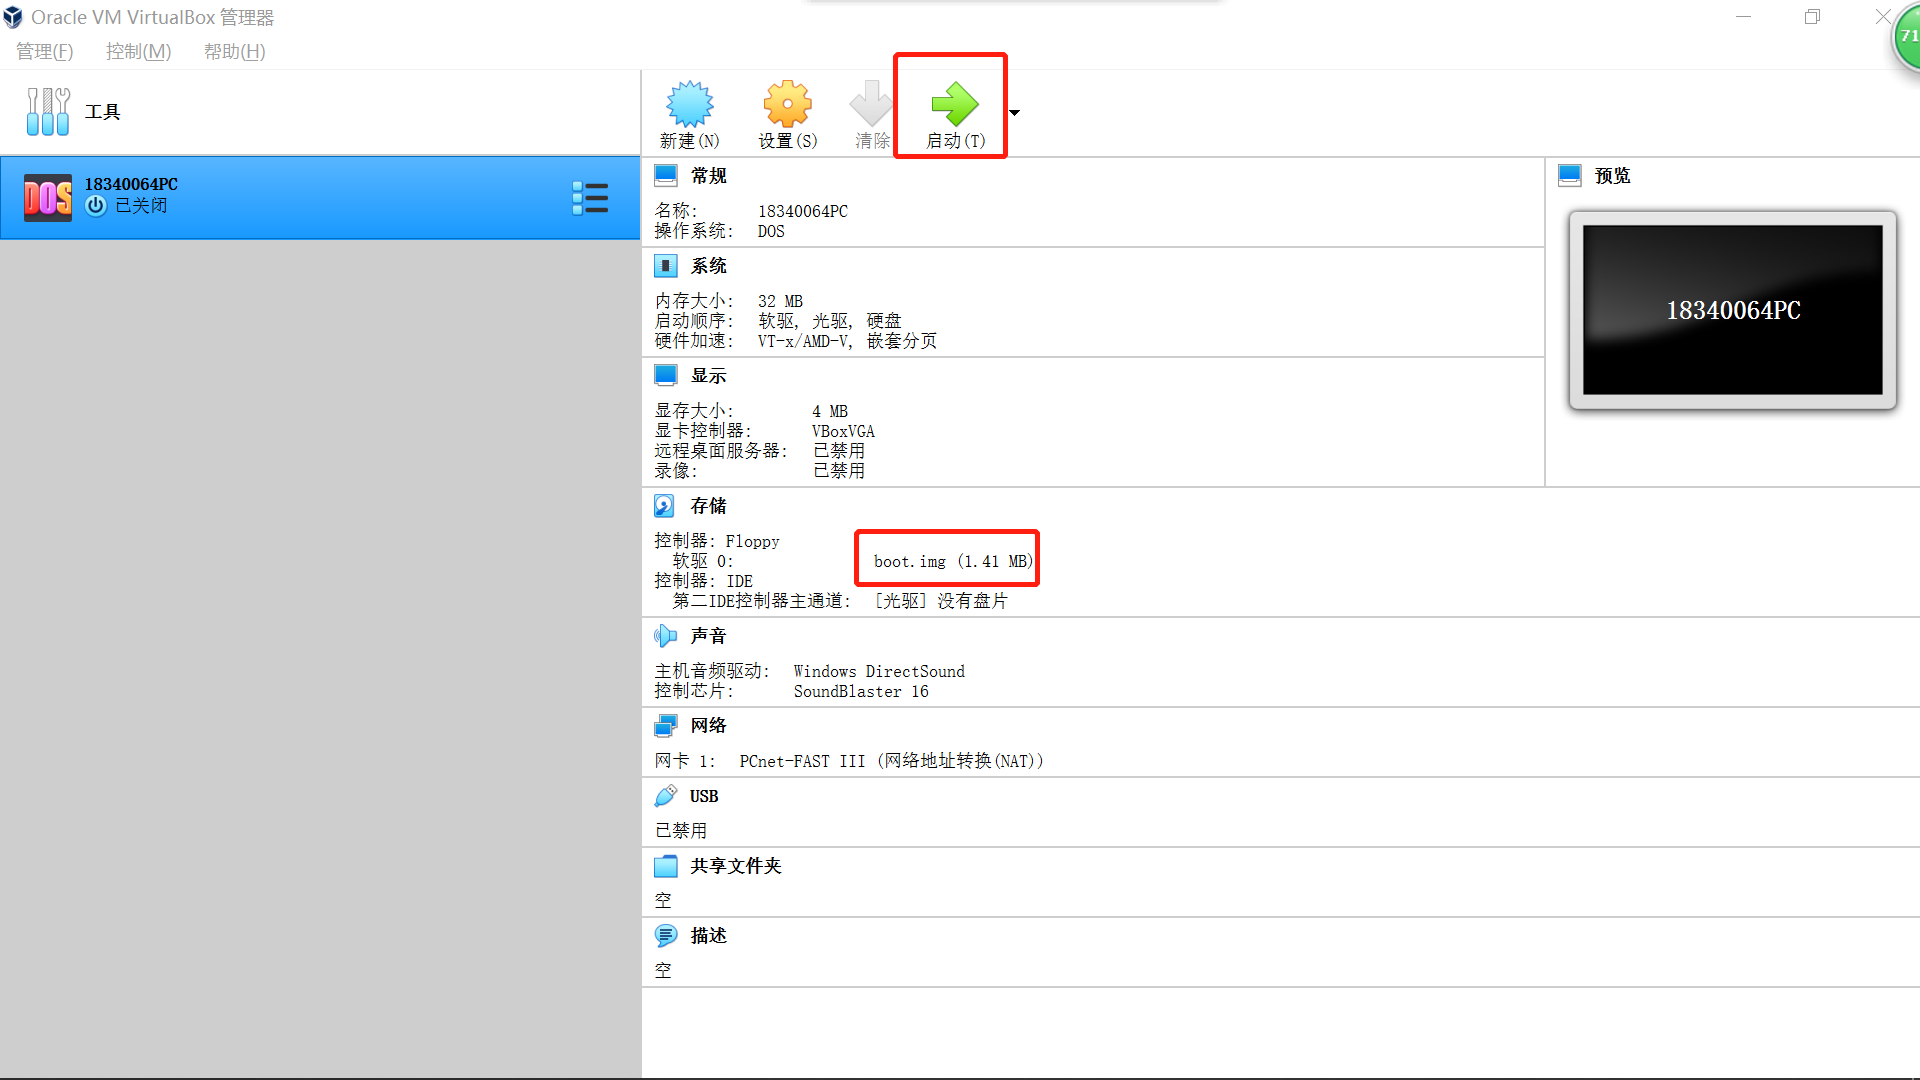
\includegraphics[width=14cm]{./figures/bootpc.png}
			\caption{设置虚拟机软驱} 
		\end{figure}	

	\begin{figure}[H]
			%\small
			\centering
			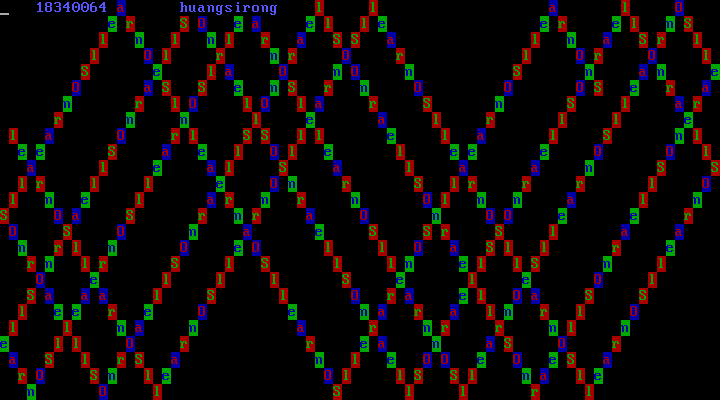
\includegraphics[width=14cm]{./figures/result.png}
			\caption{启动画面} 
		\end{figure}	

\subsection{\Large Message.img写入个人信息}
\paragraph{}\quad 使用汇编代码生成个人信息的机器码,然后写入Message.img
\begin{lstlisting}
datadef:
    number  db	'1',89h,'8',89h,'3',89h,'4',89h,'0',89h,'0',89h,'6',89h,'4',89h   ;学号
    name	db 'h',89h,'u',89h,'a',89h,'n',89h,'g',89h,'s',89h,'i',89h,'r',89h,'o',89h,'n',89h,'g',89h ;姓名
\end{lstlisting}

	\begin{figure}[H]
			%\small
			\centering
			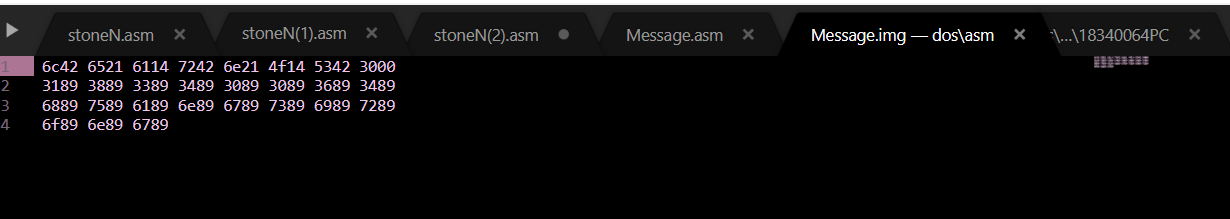
\includegraphics[width=12cm]{./figures/Message1.png}
			\caption{汇编生成的机器码} 
		\end{figure}	

	\begin{figure}[H]
			%\small
			\centering
			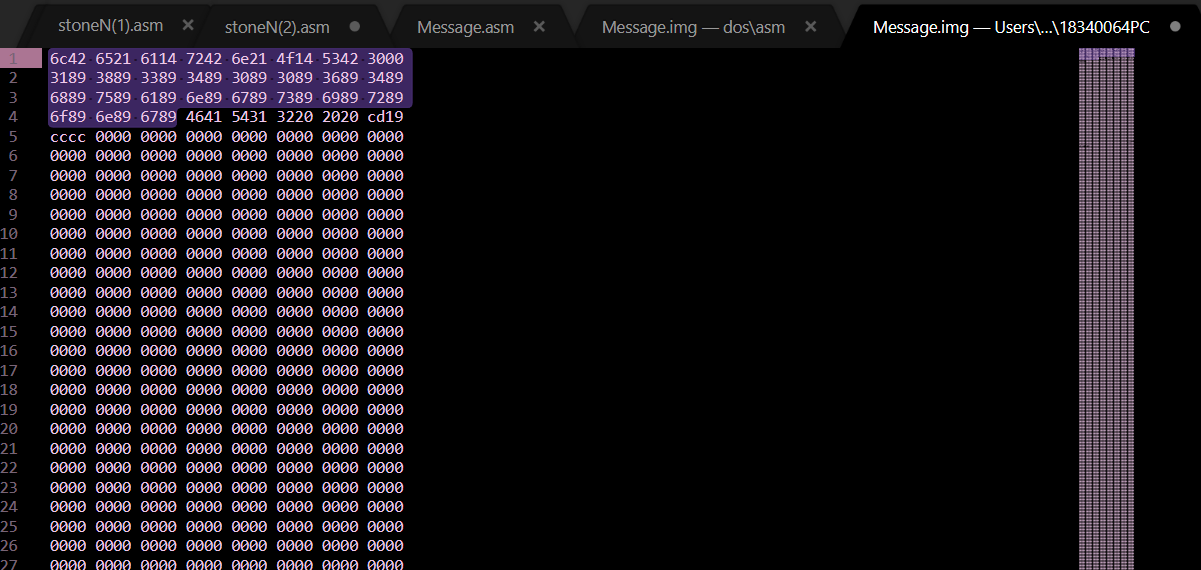
\includegraphics[width=14cm]{./figures/Message2.png}
			\caption{写入Message.img} 
		\end{figure}	

\section{\LARGE 实验总结}
\paragraph{}\quad 实验成功之后,把过程写成实验报告,回看实验报告的流程看似很简单,但
其中有很多曲折。
\paragraph{}\quad 一开始对于实验内容其实是很模糊的,主要也是因为缺乏汇编知识。在学习
计算机组成原理的时候接触的是mips指令,对于x86是不了解的,所以一开始 在看到老师的代码的时候,一来看不懂,二来直接对老师提供的代码编译会报错。
\paragraph{}\quad 所以一开始是先看了王爽的《汇编语言(第3版)》才对汇编语言有所了解,
接着也看了李忠的《x86汇编语言-从实模式到保护模式》,再回看老师提供的代 码就看懂了。
\paragraph{}\quad 不过因为王爽的汇编语言书是用 masm 的,而李忠的汇编语言书用的 nasm,一开始并不知道两者的区别,后来实践的时候就知道了……所以因为先 看的王爽的汇编书,而用 masm只能编译成.obj和.exe文件,无法直接在虚拟机 中配置使用,在这里折腾了挺久的,后来使用 nasm,可以很方便的编译成 img
或bin文件就解决问题了。 在完成了添加个人信息和字符的一些个性变化后,尝试过写如同时控制两
个运动的轨迹,写了之后感觉逻辑上是可以的,但是代码量太长了,超过了512
字节,还在想着改进办法……
\paragraph{}\quad 以及在老师修改了实验要求和内容之后,不是很明白为什么要搞三个盘,明明一个盘装引导程序的,后来想想可能是为后面的实验做准备……
\paragraph{}\quad 最后总的来说,当启动虚拟机后,看到画面的运动轨迹还是很有成就感的!
另外也要加紧汇编语言的学习!

\section{\LARGE 参考资料}
\begin{enumerate}
\item 王爽著.《汇编语言(第 3 版)》.清华大学出版社.2003 年 9 月
\item 李忠著. 《 x86 汇编语言-从实模式到保护模式》.电子工业出版社,2013 年 1 月
\item 虚拟机VirtualBox 安装教程. \url{https://blog.csdn.net/qq_33690342/article/details/81412167}
\end{enumerate}


\end{document}